\documentclass[article, 12pt, oneside, a4paper, brazil]{abntex2}

\usepackage{lmodern}
\usepackage[T1]{fontenc}
\usepackage[utf8]{inputenc}
\usepackage{lastpage}
\usepackage{indentfirst}
\usepackage{color}
\usepackage{graphicx}
\usepackage{microtype}
\usepackage{tabularx}
\usepackage{booktabs}

% Informações de dados para CAPA e FOLHA DE ROSTO
% ---
\titulo{Sistema de Pedidos Eletrônico para Restaurantes com Controle de Fluxos de Produção e Programa de Fidelidade}
\autor{Bruno Martinez da Camara \\ Douglas Juares Ortlieb \\Maria Paula Zago}
\local{Campo Mourão}
\data{\today}
\orientador{}
\coorientador{}
\instituicao{%
  Universidade Tecnológica Federal do Paraná -- UTFPR
  \par
  teste 1
  \par
  teste 2}
\tipotrabalho{teste 3}
% O preambulo deve conter o tipo do trabalho, o objetivo, 
% o nome da instituição e a área de concentração 
\preambulo{Sistema de Pedidos Eletrônico para Restaurantes com Controle de Fluxos de Produção e Programa de Fidelidade}

\definecolor{blue}{RGB}{41,5,195}

% Informações do PDF
\makeatletter
\hypersetup{
     	%pagebackref=true,
		pdftitle={\@title}, 
		pdfauthor={\@author},
    	pdfsubject={\imprimirpreambulo},
	    pdfcreator={LaTeX with abnTeX2},
		pdfkeywords={abnt}{latex}{abntex}{abntex2}{trabalho acadêmico}, 
		colorlinks=true,       		% false: boxed links; true: colored links
    	linkcolor=blue,          	% color of internal links
    	citecolor=blue,        		% color of links to bibliography
    	filecolor=magenta,      		% color of file links
		urlcolor=blue,
		bookmarksdepth=4
}
\makeatother

\setlength{\parindent}{1.3cm}
\setlength{\parskip}{0.2cm}
\makeindex

\begin{document}
\selectlanguage{brazil}
\frenchspacing

\pretextual

\imprimircapa

\pdfbookmark[0]{\contentsname}{toc}
\tableofcontents*
\cleardoublepage

\textual

 \section*{\textbf{Documento de Requisitos:} Sistema de Pedidos Eletrônico para Restaurantes com Controle de Fluxos de Produção e Programa de Fidelidade}
 \section{Introdução}
 
 \subsection{Propósito}
 O propósito deste documento de especificação de requisitos é definir todos os requisitos do Sistema de Pedidos Eletrônico para Restaurantes com Controle de Fluxos de Produção e Programa de Fidelidade, sistema que tem como objetivo principal gerenciar pedidos, controlar o fluxo de produção e informar os itens sendo produzidos aos clientes, bem como oferecer bonificações aos clientes baseado no histórico de compras.
 
 \subsection{Escopo}
 O sistema recebe os pedidos através de um atendente e os envia para a unidade produção, onde entram para o fluxo de produção de três estágios, sendo eles recebido, em produção e pronto, sendo que tais informações são compartilhadas com os clientes.
 
 \subsection{Organização da Especificação de Requisitos de Software}
 
 Este documento está dividido em três seções. Na primeira seção é apresentada uma breve introdução sobre o conteúdo deste documento. Na segunda seção, uma descrição geral do sistema é apresentada e na última seção são descritos, de forma detalhada, todos os requisitos funcionais e não-funcionais do sistema.
 
 \section{Descrição Geral do Sistema}
 O objetivo do sistema é receber os pedidos dos clientes através de um dispositivo móvel portado pelo atendente. O pedido é enviado ao sistema e é impressa uma cópia do pedido contendo os detalhes e o número da mesa do cliente.
 
 O pedido é enviado à unidade de produção através do controle de fluxo de produção e entra para o estágio recebido, assim que sua produção for iniciada, sua situação deve ser alterada para em produção e após finalizado para aguardando retirada. Tais informações também estarão disponíveis aos clientes por meio de um dispositivo de exibição. 
 
 O pedido é encerrado quando o cliente efetua o seu pagamento, a identificação é realizada pelo número da mesa que ele estava ocupando, o cliente é identificado pelo seu número do CPF (Cadastro de Pessoas Físicas) e o pedido é salvo no histórico de compras. O histórico de compras visa oferecer bonificações baseadas nas regras de negócio.
 
 \subsection{Funções do Produto}
 O sistema apresenta como principal objetivo gerenciar o ciclo de produção em um restaurante, desde a realização até o pagamento do pedido, realizando as seguintes funções:
 
 \begin{itemize}
  \item Inclusão, alteração, exclusão e consulta de ingredientes;
  \item Inclusão, alteração, exclusão e consulta de produtos;
  \item Inclusão, alteração e consulta de pedidos;
  \item Inclusão e consulta de clientes;
  \item Emissão do histórico de compras por cliente;
 \end{itemize}

 \subsection{Características do Usuário}
 O sistema é destinado a três grupos de usuários, sendo eles: atendentes, cozinheiros e caixa. O caixa desempenha também a função de gerente do sistema. Sendo necessário ter uma noção básica sobre computadores.
 
 \subsection{Suposições e Dependências}
 A configuração mínima requerida para a execução do sistema é composta por dispositivos móveis portadores de android, dois microcomputadores, sendo um com tela sensível ao toque e o outro hospedando o sistema, por fim, uma televisão para exibir o estado dos pedidos.
 
 \section{Requisitos Específicos} 
 \subsection{Requisitos Funcionais}
 
 \subsection*{\emph{Cadastro de Ingredientes}}
 \begin{description}
  \item[RF1.] O sistema deve permitir a inclusão, alteração e remoção de ingredientes no sistema. Os dados de ingredientes consistem de: nome, preço, fornecedor, contato do fornecedor e quantidade em estoque.
  \item[RF2.] O sistema deve permitir o cadastro de apenas um ingrediente por nome.
  \item[RF3.] O sistema deve permitir apenas ao administrador incluir, alterar ou remover ingredientes.
 \end{description}

 \subsection*{\emph{Cadastro de Produtos}}
 \begin{description}
  \item [RF4.] O sistema deve permitir a inclusão, alteração e remoção de produtos no sistema. Os dados de produtos consistem de: número de identificação único, nome, preço, ingredientes e categoria.
  \item [RF5.] O sistema deve permitir a alteração dos dados do produto, exceto o número de identificação único.
  \item [RF6.] O sistema não deve permitir que produtos com falta de ingredientes sejam adicionados aos pedidos.
  \item [RF7.] O sistema deve permitir apenas ao administrador incluir, alterar ou remover produtos.
 \end{description}
 
 \subsection*{\emph{Cadastro de Pedidos}}
 \begin{description}
  \item [RF8.] O sistema deve permitir a inclusão e alteração dos pedidos. Os dados de pedido consistem de: número do pedido, produtos, valor total, identificação do cliente, data do pedido e estado do pedido.
  \item [RF9.] O sistema deve permitir a alteração dos dados do pedido, exceto o número do pedido, a identificação do cliente e a data do pedido.
  \item [RF10.] O sistema deve permitir a alteração do campo estado do pedido para: recebido, em produção, aguardando retirada e finalizado.
  \item [RF11.] O sistema deve permitir a inclusão de itens adicionais ao pedido.
 \end{description}
 
 \subsection*{\emph{Cadastro de Clientes}}
 \begin{description}
  \item [RF12.] O sistema deve permitir a inclusão de clientes. Os dados de clientes consistem de: CPF, nome do cliente e pontos acumulados.
  \item [RF13.] O sistema deve permitir o cadastro de apenas um cliente por CPF.
 \end{description}
 
 \subsection*{\emph{Informações do Programa de Fidelidade}}
 \begin{description}
  \item [RF14.] O sistema deve permitir que um pedido esteja vinculado a apenas um cliente.
  \item [RF15.] O sistema deve permitir que apenas pedidos com o estado de finalizados sejam vinculados aos pontos acumulados do cliente.
 \end{description}
 
 \subsection*{\emph{Relatórios}}
 \begin{description}
  \item [RF16.] O sistema deve gerar relatórios de todos os pedidos realizados por cliente, data ou produto.
  \item [RF17.] O sistema deve gerar relatórios da quantidade de ingredientes em estoque.
 \end{description}
 
 \subsection{Requisitos Não-Funcionais}
 \begin{description}
  \item [RN1.] O sistema é composto por quatro (4) subsistemas, sendo eles: sistema para atendimento, sistema para fluxo de produção, sistema para caixa e sistema para administração.
  \item [RN2.] O sistema deve ser capaz de realizar cópias de segurança e restauração de todos os dados do sistema.
  \item [RN3.] O sistema deve ser facilmente portável para os ambientes Linux e Windows.
 \end{description}

  \pagebreak
 
 \section{Diagramas de Caso de Uso}
 \subsection{Diagrama de Caso de Uso Para Pedidos}
 \begin{figure}[!htb]
 \caption{Diagrama de Caso de Uso Para Pedidos}
 \begin{center}
 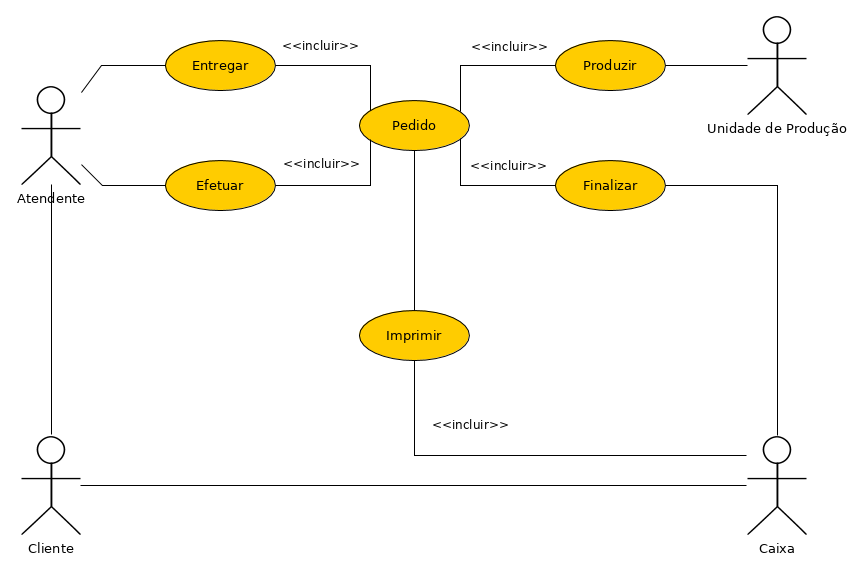
\includegraphics[width=\textwidth]{images/pedidos001.png}
 \end{center}
 \end{figure}
 
 \section{Descrição Casos de Uso}
 
 \subsection{Descrição Resumida dos Casos de Uso}
 
 \subsubsection{Descrição Resumida do Caso de Uso Efetuar Pedido}
 
\begin{table}[!htb]
\caption{Descrição Resumida do Caso de Uso Efetuar Pedido}
 \begin{center}
  \begin{tabularx}{\textwidth}{lX}\specialrule{1.2pt}{1pt}{1pt}
  \textbf{Caso de Uso:} & Efetuar Pedido\\ \hline
  \textbf{Visão Geral:} & O cliente realiza o pedido dos itens desejados ao atendente e o sistema  registra o pedido. Após o registro, uma cópia do  pedido é impressa e retira no caixa.\\ \specialrule{1.2pt}{1pt}{1pt}
  \end{tabularx}
 \end{center}
\end{table}

\pagebreak
 \subsubsection{Descrição Resumida do Caso de Uso Produzir Pedido}
 
\begin{table}[!htb]
\caption{Descrição Resumida do Caso de Uso Produzir Pedido}
\begin{center}
 \begin{tabularx}{\textwidth}{lX}\specialrule{1.5pt}{1pt}{1pt}
  \textbf{Caso de Uso:} & Produzir pedido\\ \hline
  \textbf{Visão Geral:} & O sistema envia o pedido à cozinha onde tem o seu estado atualizado de acordo com o fluxo de produção. O pedido entra automaticamente com o estado de recebido, ao iniciar a produção tem o estado alterado para em produção e após terminado o processo para pronto/aguardando retirada.\\ \specialrule{1.5pt}{1pt}{1pt}
 \end{tabularx}
\end{center}
\end{table}

\subsubsection{Descrição Resumida do Caso de Uso Entregar Pedido}

\begin{table}[!htb]
\caption{Descrição Resumida do Caso de Uso Entregar Pedido}
\begin{center}
 \begin{tabularx}{\textwidth}{lX}\specialrule{1.2pt}{1pt}{1pt}
  \textbf{Caso de Uso:} & Entregar pedido\\ \hline
  \textbf{Visão Geral:} & Quando finalizado, o produto é entregue ao cliente pelo atendente ou o próprio cliente o retira identificando o número da mesa. O sistema atualiza o estoque baseado nos itens do pedido. \\ \specialrule{1.2pt}{1pt}{1pt}
 \end{tabularx}
\end{center}
\end{table}

\subsubsection{Descrição Resumida do Caso de Uso Finalizar Pedido}

\begin{table}[!htb]
\caption{Descrição Resumida do Caso de Uso Finalizar Pedido}
\begin{center}
 \begin{tabularx}{\textwidth}{lX}\specialrule{1.2pt}{1pt}{1pt}
  \textbf{Caso de Uso:} & Finalizar Pedido\\ \hline
  \textbf{Visão Geral:} & O cliente dirige-se ao caixa, informa o número da mesa em que está e o seu CPF, o caixa informa os dados ao sistema, o sistema identica o cliente e o pedido, e informa as bonificações disponíveis, o cliente efetua o pagamento e o sistema finaliza o pedido. Após finalizado o sistema imprime um cupom fiscal contendo os detalhes do pedido e o número de pontos no programa recompensa. \\ \specialrule{1.2pt}{1pt}{1pt}
 \end{tabularx}
\end{center}
\end{table}

\pagebreak

\subsection{Descrição Completa Abstrata dos Casos de Uso}

\subsubsection{Descrição Completa e Abstrata do Caso de Uso Realizar Pedido}

\begin{table}[!htb]
\caption{Descrição Completa e Abstrata do Caso de Uso Realizar Pedido}
\begin{center}
 \begin{tabularx}{\textwidth}{lX}\specialrule{1.2pt}{1pt}{1pt}
  \textbf{Descrição:} & Este caso de uso detalha como é realizada a inclusão de um pedido realizado pelo cliente no sistema.\\ \hline
  \textbf{Atores:} & Atendente.\\ \hline
  \textbf{Inclusões:} & Imprimir Pedido, Alterar Pedido.\\ \hline
  \textbf{Extensões:} & Nenhuma.\\ \hline
  \textbf{Pré-condições:} & O atendente deve informar ao sistema a mesa do cliente. \\ \hline
  \textbf{Detalhes:} & \begin{enumerate}[wide, labelwidth=!, noitemsep]
                           \item O atendente inclui no pedido os itens informados pelo cliente.
                           \item O atendente finaliza o pedido.
                           \item O sistema registra o pedido.
                           \item A impressora imprime um comprovante contendo os itens do pedido.
                           \item O comprovante é retido no caixa.
                          \end{enumerate}
\\ \hline
  \textbf{Pós-condições:} & O pedido estará registrado no sistema e com estado de recebido. \\ \hline
  \textbf{Exceções:} & O cliente cancela o pedido.\\ \hline
  \textbf{Restrições:} & O item que o cliente solicitou está indisponível. \\ \hline
  \textbf{Variantes:} & Nenhuma.\\ \hline
  \textbf{Comentários:} &  O pedido deve ser realizado somente pelo atendente. Enquanto o pedido estiver com estado de produção é possível alterá-lo.\\ \specialrule{1.2pt}{1pt}{1pt}
 \end{tabularx}
\end{center}
\end{table}

\pagebreak

\subsubsection{Descrição Completa e Abstrata do Caso de Uso Produzir Pedido}

\begin{table}[!htb]
\caption{Descrição Completa e Abstrata do Caso de Uso Produzir Pedido}
\begin{center}
 \begin{tabularx}{\textwidth}{lX}\specialrule{1.2pt}{1pt}{1pt}
  \textbf{Descrição:} & Este caso de uso detalha como é realizada a produção de um pedido.\\ \hline
  \textbf{Atores:} & Unidade de produção.\\ \hline
  \textbf{Inclusões:} & Nenhuma.\\ \hline
  \textbf{Extensões:} & Nenhuma.\\ \hline
  \textbf{Pré-condições:} & O sistema deve ter pelo menos um pedido com estado de recebido. \\ \hline
  \textbf{Detalhes:} & \begin{enumerate}[wide, labelwidth=!, noitemsep]
                           \item A unidade de produção recebe o pedido no sistema de fluxo de produção.
                           \item A unidade de produção seleciona o pedido.
                           \item O sistema altera o estado do pedido para em produção.
                           \item A unidade de produção inicia a produção do item.
                           \item A unidade de produção termina a produção do item.
                           \item O sistema altera o estado do pedido para pronto.
                          \end{enumerate}
\\ \hline
  \textbf{Pós-condições:} & O item está pronto e aguardando retirada. \\ \hline
  \textbf{Exceções:} & Nenhuma.\\ \hline
  \textbf{Restrições:} & Nenhuma. \\ \hline
  \textbf{Variantes:} & 2.1. Caso não possa ser produzido imediatamente, o pedido continua no mesmo estado.\\ \hline
  \textbf{Comentários:} &  O sistema deve priorizar os pedidos mais antigos.\\ \specialrule{1.2pt}{1pt}{1pt}
 \end{tabularx}
\end{center}
\end{table}

\pagebreak

\subsubsection{Descrição Completa e Abstrata do Caso de Uso Entregar Pedido}

\begin{table}[!htb]
\caption{Descrição Completa e Abstrata do Caso de Uso Entregar Pedido}
\begin{center}
 \begin{tabularx}{\textwidth}{lX}\specialrule{1.2pt}{1pt}{1pt}
  \textbf{Descrição:} & Este caso de uso detalha como é realizada a entrega de um pedido.\\ \hline
  \textbf{Atores:} & Atendente.\\ \hline
  \textbf{Inclusões:} & Nenhuma.\\ \hline
  \textbf{Extensões:} & Nenhuma.\\ \hline
  \textbf{Pré-condições:} & O pedido deve estar no estado pronto. \\ \hline
  \textbf{Detalhes:} & \begin{enumerate}[wide, labelwidth=!, noitemsep]
                           \item O atendente retira o pedido do balcão.
                           \item O atendente entrega o pedido na mesa correspondente.
                           \item O estado do pedido é alterado para entregue.
                           \item O estoque é atualizado.
                          \end{enumerate}
\\ \hline
  \textbf{Pós-condições:} & O item produzido deve estar de acordo com o pedido. O estoque deve estar atualizado com os novos valores.\\ \hline
  \textbf{Exceções:} & Nenhuma.\\ \hline
  \textbf{Restrições:} & Nenhuma. \\ \hline
  \textbf{Variantes:} & Nenhuma.\\ \hline
  \textbf{Comentários:} &  O pedido pode ter seus itens entregues parcialmente.\\ \specialrule{1.2pt}{1pt}{1pt}
 \end{tabularx}
\end{center}
\end{table}

\pagebreak

\subsubsection{Descrição Completa e Abstrata do Caso de Uso Finalizar Pedido}

\begin{table}[!htb]
\caption{Descrição Completa e Abstrata do Caso de Uso Finalizar Pedido}
\begin{center}
 \begin{tabularx}{\textwidth}{lX}\specialrule{1.2pt}{1pt}{1pt}
  \textbf{Descrição:} & Este caso de uso detalha como é finalizado um pedido.\\ \hline
  \textbf{Atores:} & Caixa.\\ \hline
  \textbf{Inclusões:} & Nenhuma.\\ \hline
  \textbf{Extensões:} & Nenhuma.\\ \hline
  \textbf{Pré-condições:} & Todos os itens do pedido devem ter sido entregues corretamente. \\ \hline
  \textbf{Detalhes:} & \begin{enumerate}[wide, labelwidth=!, noitemsep]
                           \item O cliente informa o número da mesa e o CPF.
                           \item O caixa informa esses dados ao sistema.
                           \item O sistema exibe o pedido e as informações do cliente ao caixa.
                           \item O caixa informa ao cliente o valor do pedido incluindo os descontos do programa de fidadelidade.
                           \item O cliente efetua o pagamento.
                           \item O caixa encerra o pedido.
                           \item O sistema imprime o cupom fiscal.
                           \item O cumpom fiscal é entregue ao cliente contendo a pontução do sistema de recompensa.
                           \item O sistema altera o estado do pedido para finalizado.
                          \end{enumerate}
\\ \hline
  \textbf{Pós-condições:} & O sistema deve registrar os dados do pedido. Caso o cliente participe do programa de fidelidade deve ter os pontos creditados ao seu cadastro.\\ \hline
  \textbf{Exceções:} & Nenhuma.\\ \hline
  \textbf{Restrições:} & O pedido não pode ser fechado caso não haja o pagamento integral do valor. \\ \hline
  \textbf{Variantes:} & \begin{enumerate}[wide, labelwidth=!, noitemsep]
                           \item[3.1.] O sistema exibe o pedido ao caixa e informa que o cliente não é cadastrado.
                           \item[3.2.a.] O cliente informa seus dados ao caixa.
                           \item[3.2.b.] O cliente não tem interesse em realizar o cadastro.
                           \item[3.3.a.] O caixa cadastra o cliente no sistema.
                           \item[4.1.b.] O caixa informa ao cliente o valor do pedido.
                           \item[7.1.b.] O cumpom fiscal é entregue ao cliente.
                          \end{enumerate}\\ \hline
  \textbf{Comentários:} &  É opcional ao cliente utilizar os pontos do programa de recompensa.\\ \specialrule{1.2pt}{1pt}{1pt}
 \end{tabularx}
\end{center}
\end{table}

\end{document}
